\documentclass[fleqn,10pt]{wlscirep}
\usepackage[utf8]{inputenc}
\usepackage[T1]{fontenc}
\usepackage{graphicx}
\usepackage[section]{placeins}
\usepackage{url}

% Round-1 revision marker: wraps text added/changed in this revision so the
% co-author can review the deltas in blue. Strip after review by redefining
% to identity: \renewcommand{\rev}[1]{#1}
\newcommand{\rev}[1]{\textcolor{blue}{#1}}

% Clickable cross-reference to the (unnumbered) Methods section, matching
% the behavior of table/figure references.
\newcommand{\Methods}{\hyperref[sec:methods]{Methods}}

\title{Neural-network placement in physics-informed machine learning for mechanistic process-model repair: a case study in industrial coffee roasting}

\author[1,*]{Morgen Pronk}
\author[1,*]{Brian W. Anthony}
\affil[1]{Massachusetts Institute of Technology, Cambridge, MA, USA}
\affil[*]{morgenpronk@alum.mit.edu; banthony@mit.edu}

\begin{abstract}

Mechanistic process models are central to industrial simulation and control, but their rollout accuracy often depends on run-specific initialization data that archival production telemetry cannot reliably provide. This gap can leave predictions inaccurate even when the underlying physical scaffold is approximately correct. Physics-informed machine learning (PIML) can be used to repair such models from data, yet many comparisons do not isolate a key design choice: where the learned neural network is placed relative to the mechanistic ordinary differential equation (ODE). Using a 221-roast industrial coffee-roasting cohort, this study compares four PIML repair strategies and a matched-input neural baseline as a six-model placement spectrum, holding the learned network family fixed (feedforward multilayer perceptron, MLP) so that the primary design variable is neural-network placement rather than neural architecture. The four PIML strategies lift autonomous-rollout R² from -0.44 to 0.70-0.94; the matched-input neural baseline reaches 0.97 with 3-20 times fewer parameters than every PIML strategy tested. Three structural findings characterize the spectrum. First, the PIML strategies tend to share their hard roasts (per-roast Pearson r approximately 0.5-0.9), whereas the neural baseline identifies a different set of hard roasts (r approximately 0), reaching a comparable predictive ceiling through structurally different failure profiles. Second, in this benchmark a physics-motivated bound on the residual correction costs more than it buys: the unbounded variant uses 3.7 times fewer parameters while improving R² by 0.02. Third, seed stability varies by more than an order of magnitude across PIML strategies \rev{(range 0.009 to 0.117 R² across five or more retraining seeds)}.

These findings suggest that, for this metadata-limited cohort, physics-informed scaffolds are effective repair mechanisms for mechanistic rollouts, but they do not automatically provide better parameter efficiency or optimization stability than a compact matched-input empirical baseline.

\end{abstract}

\begin{document}
\flushbottom
\maketitle
\thispagestyle{empty}

\section*{Introduction}

\rev{Industrial production processes are often governed by well-established physical laws, yet the run-specific information a mechanistic model requires is rarely fully recorded: material properties, operating conditions at the start of a run, and initial values of unobserved latent states are often guessed, estimated, or absent in archival production records~\cite{ljung1999,pillonetto2025}, a pattern reported across process industries, including bioreactor cultivation, semiconductor process control, polymer extrusion, and food processing. A model built on such records must fall back on literature priors or infer its initialization from startup observables, and priors matched to the specific machine, material, and operating regime are often no more available than the measurements. When initialization fails by either route, the mechanistic rollout can drift even when the underlying physics is approximately correct.} This trajectory-deficit failure mode is the specific setting in which physics-informed machine learning \rev{(PIML, used here in the broad hybrid-modeling sense~\cite{karniadakis2021,schweidtmann2024})} is evaluated here.

Several hybrid and physics-informed strategies have been proposed for this purpose: learning unresolved closure terms within the mechanistic ODE while preserving its structure---an approach first introduced by Psichogios and Ungar~\cite{psichogios1992} and developed across the hybrid semi-parametric literature~\cite{vonStosch2014,karniadakis2021,rackauckas2020universal}; adding residual neural corrections on top of a mechanistic rollout~\cite{kennedy2001bayesian,vonStosch2014}; or training matched-input neural sequence models without a mechanistic scaffold~\cite{ljung1999,pillonetto2025}. These strategies are individually well established and sit within a developed hybrid-modeling taxonomy~\cite{vonStosch2014,sansana2021,sharma2022,rajulapati2022,schweidtmann2024}. This framing is also distinct from classical physics-informed neural networks~\cite{raissi2019}, which impose physical laws via residual loss terms on a continuous-time PDE solution; the present work instead places learned components around a discrete-time mechanistic ODE rollout. \rev{Similar strategies appear beyond the process industries, in environmental modeling~\cite{read2019} and across the applications catalogued in surveys of science-guided machine learning~\cite{willard2022}; in most of these studies, however, the placement of the learned component is fixed by design rather than treated as the variable under test.} Comparative studies on shared datasets are beginning to appear: Jul-Rasmussen et al.~\cite{julrasmussen2025} recently benchmarked a serial hybrid semi-parametric model against physics-informed recurrent neural networks (PIRNNs) and a purely data-driven recurrent baseline on pilot-scale bubble column aeration data, finding the hybrid semi-parametric approach generally superior; and within the neural-ODE strand, Sorourifar et al.~\cite{sorourifar2023} introduced a physics-enhanced NODE framework that varies the level of mechanistic prior knowledge embedded in the ODE right-hand side. The contribution of this paper is therefore narrower and more specific: a like-for-like, validation-selected comparison of four repair strategies against an unconstrained neural baseline, organized as a placement spectrum in which six model classes are arrayed by where the learned MLP sits relative to the mechanistic ODE. The practical question for system identification on metadata-limited production data is not whether PIML can be beneficial in principle, but which repair position is most effective in practice and how it compares with a compact empirical baseline that does not attempt to repair the physics. \rev{The intended scope is correspondingly narrow: a within-configuration comparison on a single industrial roaster and three recurring roast labels; transfer across machines, recipes, or bean varieties lies outside the validated scope and is addressed only as future work.}

Industrial coffee roasting is a useful case study for this comparison because two lines of evidence support, but do not by themselves prove, the adequacy of the underlying physical scaffold in the regime studied here. First, the model form is grounded in a substantial heat- and mass-transfer literature for bean temperature evolution~\cite{schwartzberg2002,vosloo2017,putranto2012,hernandez2007,fabbri2011,fadai2017}, with recent extensions to alternative roaster geometries~\cite{alshemmeri2025}. Second, the parameterization is supported empirically on this cohort: when literature values for the kinetic and heat-transfer parameters are used and only small data-driven corrections are fitted on top of them, the published ODE reproduces these trajectories at rollout $R^2$ approximately $0.93$ (verified in \Methods). Together, these observations make missing run-specific initialization a plausible dominant source of rollout failure in the experimental regime evaluated below, rather than requiring a claim that model-form or parameter error is absent. Thus, the experiment does not ask whether a fully anchored literature model can be improved from an already high $R^2$ approximately $0.93$ baseline; it asks how different PIML plug-in positions repair the more common production-data regime in which the ODE form is credible but run-specific initialization and anchoring metadata are unavailable.

Starting from the priors-equipped $R^2$ approximately $0.93$ model would leave little dynamic range for comparing repair strategies. This work therefore evaluates the metadata-limited variant: the same mechanistic scaffold is used, but run-specific latent initialization and anchoring priors are not supplied. This design isolates the repair role of PIML under a failure mode that is common in archival industrial telemetry.

The placement spectrum spans six model classes. The first two place learned MLPs \emph{inside} the mechanistic ODE: a single-closure variant that replaces only the heat-transfer coefficient $h_e$ with a learned function of measured drivers, and a multi-closure variant that additionally replaces the moisture-loss and exothermic reaction rates with bounded learned MLPs. The next two repair strategies place a learned MLP \emph{on top of} the mechanistic rollout as an additive correction: a bounded variant in which the correction is constrained to a small temperature-space neighborhood of the mechanistic prediction, and an unbounded variant in which the correction is free. The comparator is a matched-input feedforward neural baseline that operates on the same measured drivers as the repair strategies but uses no mechanistic scaffold. Every learned component in the comparison is a feedforward MLP with hidden architecture selected independently for each class by validation-rollout random search; the comparison axis is therefore where the MLP plugs in relative to the mechanistic ODE, not what kind of network is used.

Each model class is independently tuned over a 40-trial sweep and retrained at a shared training budget across \rev{five or six retraining seeds} on a 221-roast production cohort with deterministic whole-roast hash splits. The comparison characterizes each repair method along five axes: autonomous-rollout $R^2$ on held-out roasts, parameter efficiency, training cost, seed-to-seed reproducibility, and per-roast failure-mode structure. The findings are intended to guide method choice for hybrid physics-informed system identification on production data where reliable run-specific metadata is unavailable.

\section*{Results}

On rollout accuracy alone, the strongest PIML repairs and the neural baseline have overlapping bootstrap confidence intervals, while the neural baseline reaches the highest point estimate with 3 to 20 times fewer parameters, faster training, and a different per-roast failure pattern.

\subsection*{A metadata-indexed production cohort anchors the comparison}

Held-out evaluation used a fixed 221-roast production cohort drawn from one source bucket and three recurring roast labels. After trimming each roast to the bean-charge-to-dump modeled window, deterministic whole-roast hash splitting produced 150 training roasts, 35 validation roasts, and 36 held-out test roasts. The trimmed sequences had a mean modeled length of 68.4 samples, for 15,113 total modeled steps. No rows from a held-out roast appeared in training or validation. All rollout metrics below are reported on the held-out test roasts.

\subsection*{The six-class placement spectrum at a glance}

Table~\ref{tab:rollout_summary} summarizes held-out rollout performance for all six model classes, ordered by where the learned MLP attaches to the mechanistic ODE: nowhere (row 1, the mechanistic baseline), inside the ODE as one or three learned closures (rows 2--3), on top of the ODE rollout as a bounded or unbounded additive correction (rows 4--5), and standalone with no scaffold (row 6). The table reports the seed-11 held-out rollout $R^2$ with bootstrap CI, root-mean-square error (RMSE), and trainable-parameter count for each class; Figure~\ref{fig:position_spectrum} reproduces the same accuracy axis alongside per-seed reproducibility across \rev{all evaluated retraining seeds (five per class, six where available; \Methods)} and parameter count on log scale. \rev{All symbols used in the Results are defined in Table~\ref{tab:symbols} and in \Methods.} The subsections that follow walk through each repair group in turn (in-scaffold, on top of the rollout, standalone), then return to the cross-class structural findings on seed stability and per-roast failure-mode correlation.

\subsection*{Learned closures inside the ODE repair the rollout}

The single-closure \rev{physics-informed (PI) variant} (row 2 of Table~\ref{tab:rollout_summary}) is the simplest in-scaffold repair: it replaces the constant heat-transfer coefficient $h_e$ with a learned MLP on $(T_g, v_g, T_T)$, leaving the rest of the mechanistic state evolution intact. This single-closure repair lifts rollout $R^2$ from $-0.4376$ to $0.7027$ with bootstrap interval $[0.6480,\,0.7611]$, and reduces RMSE to 19.00~$^\circ$C. The repair is statistically separated from the mechanistic baseline but well below the unconstrained neural-baseline ceiling reported below.

The multi-closure PI (row 3) extends the same in-scaffold strategy to learn three physical relations simultaneously (the heat-transfer closure $h_e$, the moisture-loss rate $\dot{X}_b$, and the exothermic reaction rate $\dot{H}_e$), raising rollout $R^2$ to $0.9436$ with bootstrap interval $[0.9165,\,0.9717]$ and RMSE 8.28~$^\circ$C. Each rate is replaced by a bounded feedforward MLP that produces a non-positive (moisture) or non-negative (reaction) rate scaling the mechanistic default at zero-initialization. The substantial improvement over single-closure repair ($+0.24$ R$^2$ at the same training budget) is consistent with the interpretation that the moisture and reaction kinetics, not only the heat-transfer relation, contribute to the mechanistic baseline's rollout drift on this cohort.

Multi-closure repair, however, comes with wider seed sensitivity (Figure~\ref{fig:position_spectrum}). \rev{Across six retraining seeds the test rollout $R^2$ ranges from $0.8265$ to $0.9437$ (range $0.117$), with one of six seeds finishing far below the others. The single-closure repair is more stable (range $0.073$ across the same six seeds),} consistent with the increased training-dynamics interactions that arise when three coupled rate closures are learned jointly.

\subsection*{Residual corrections on top of the ODE rollout repair from outside the scaffold}

The on-top repair strategy (rows 4--5 of Table~\ref{tab:rollout_summary}) leaves the mechanistic ODE unchanged and learns an additive correction $\delta_t$ applied to the rollout's predicted temperature at each step. The correction is produced by a feedforward MLP whose inputs are the current corrected temperature and the same measured drivers $(T_2, v_g, T_T)$ used by the neural baseline below. Two variants are reported (equation~\eqref{eq:residual}): a bounded residual where the correction is constrained to a small additive perturbation of the mechanistic rollout, and an unbounded residual where the correction can override the mechanistic prediction.

The bounded residual repair reaches rollout $R^2 = 0.8963$ with bootstrap interval $[0.8566,\,0.9386]$ and RMSE 11.23~$^\circ$C; the bound (selected as $\pm 24$~K by the validation-rollout sweep) constrains the learned correction to remain a small perturbation of the mechanistic rollout rather than a free prediction. The unbounded residual repair, evaluated under the same architecture-family search space but with the bound removed, reaches $R^2 = 0.9158$ with bootstrap interval $[0.8869,\,0.9468]$ and RMSE 10.11~$^\circ$C. The unbounded variant therefore achieves higher predictive accuracy than the bounded variant, and it does so with substantially fewer learned parameters (2{,}433 vs 8{,}961, a 3.7-fold reduction). This result is consistent with the bound requiring additional model capacity to remain close to the mechanistic prediction while still achieving a similar trajectory; relaxing the bound lets the model find a more compact solution. Both residual variants are highly seed-stable: \rev{across the five valid retraining seeds (\Methods), the bounded variant has a seed-stability range of $0.018$ and the unbounded variant a range of $0.009$, the two tightest of any model class in the spectrum.}

\subsection*{The matched-input neural baseline reaches the predictive ceiling}

The matched-input neural baseline (row 6 of Table~\ref{tab:rollout_summary}) is a feedforward MLP that operates on the same measured drivers as the physics-informed model (previous $T_c$, inlet-air temperature $T_2$, air speed $v_g$, and drum speed $T_T$) and predicts the next $T_c$ directly with no mechanistic scaffold. On this cohort it reaches rollout $R^2 = 0.9697$ with bootstrap interval $[0.9560,\,0.9805]$, the highest of any model in the comparison.

After hyperparameter selection, the matched-input baseline that wins on the validation split is a compact two-hidden-layer MLP $(32 \rightarrow 16)$ with only 705 trainable parameters, more than an order of magnitude smaller than either the single-closure physics-informed MLP (11{,}250 parameters) or the multi-closure physics-informed model (14{,}196 parameters), and somewhat smaller than the bounded FF residual (8{,}961 parameters). The smallest architecture in the search space was therefore selected for the neural baseline, and it still exceeds the predictive performance of every physics-informed repair configuration on the cohort's held-out test split. The parameter-efficiency comparison runs in the opposite direction from the usual physics-informed motivation.

Compared with the strongest physics-informed repair (multi-closure, $R^2 = 0.9436$), the neural baseline's median roast-level advantage is small in absolute terms: a paired Wilcoxon signed-rank test on per-roast rollout $R^2$ yields $p = 0.32$, and a two one-sided tests (TOST) equivalence test at $\varepsilon = 0.02$ gives $p = 0.27$. The two models are neither significantly different on median per-roast performance nor formally equivalent within $\pm 0.02$ R$^2$. Compared with the single-closure repair ($R^2 = 0.7027$), the baseline outperforms on all 36 held-out roasts (paired Wilcoxon $p = 2.91 \times 10^{-11}$).

\subsection*{Seed stability differs sharply across repair strategies}

\rev{Seed-to-seed stability varies sharply across the spectrum. Figure~\ref{fig:position_spectrum} (middle panel) plots every per-seed $R^2$ value across retraining seeds (five per class, six where available; \Methods) with the per-class range annotated. The two residual variants are the most reproducible, with observed ranges of $0.009$ and $0.018$; the matched-input neural baseline follows at $0.028$. Inside the scaffold, the single-closure PI spans $0.073$ and the multi-closure PI $0.117$, with one of six seeds finishing far below the others as discussed above. The mechanistic baseline is by far the least stable, with a range of $1.23$: training diverged before convergence in every seed, so each per-seed value is a best pre-divergence checkpoint; the initialization mechanism behind this instability is detailed in \hyperref[sec:model_classes]{Model classes} (\Methods).} These values identify practical optimization sensitivity rather than a fully sampled distribution over random initializations.

\subsection*{Repair strategies and the neural baseline reach the same R$^2$ ceiling through different per-roast failure modes}

Per-roast Pearson correlations between the top trial of each class (seed 11) characterize how the strategies fail differently even when they achieve similar overall R$^2$. The four physics-informed repairs intercorrelate strongly with one another on per-roast scores: single-closure vs multi-closure $r = +0.59$, single-closure vs bounded FF residual $r = +0.92$, single-closure vs unbounded FF residual $r = +0.78$, multi-closure vs bounded FF residual $r = +0.65$, multi-closure vs unbounded FF residual $r = +0.53$, bounded vs unbounded FF residual $r = +0.94$. All these positive correlations reflect a shared mechanistic-scaffold failure-mode pattern. The matched-input neural baseline, by contrast, has near-zero per-roast correlation with every physics-informed repair (single-closure: $r = -0.01$; multi-closure: $r = -0.17$; bounded FF residual: $r = -0.03$; unbounded FF residual: $r = -0.01$). Same predictive ceiling, structurally different per-roast failure profiles. The physics-informed repairs share their hard roasts with one another; the neural baseline finds different roasts hard (Figure~\ref{fig:per_roast_corr}). Representative held-out rollouts for all six model classes on the deterministic-longest test roast are shown in Figure~\ref{fig:representative_rollouts}.

\section*{Discussion}

\rev{In this production cohort, each of the four PIML repair strategies recovers substantial predictive trajectory fidelity from the metadata-limited mechanistic baseline.} Multi-closure repair and the unbounded FF residual reach within approximately $0.05$ R$^2$ of the matched-input neural baseline; single-closure repair and bounded residual repair recover smaller but still substantial fractions of the gap. Because all four repairs use feedforward MLPs in different positions relative to the mechanistic ODE, the comparison isolates placement more than architecture. \rev{These results support a practical conclusion:} physics-informed scaffolding consistently repairs the mechanistic rollout, but none of the tested repair strategies provides a parameter-efficiency or compute-efficiency advantage over a compact unconstrained neural baseline on this cohort.

The four PIML repair strategies differ in informative ways. \emph{In-scaffold} learning (positions 2 and 3) keeps the mechanistic ODE structurally intact and replaces one or three physical rate relations with bounded learned MLPs. \rev{The gain from single- to multi-closure repair (Table~\ref{tab:rollout_summary}) indicates that the mechanistic model's error is spread across several of its empirical relations (heat transfer, moisture loss, and reaction rate) rather than concentrated in any single one.} \rev{The cost of multi-closure repair appears to be increased seed sensitivity: the multi-closure variant shows the widest per-seed range of any repair, including one seed far below the rest (Figure~\ref{fig:position_spectrum}, middle panel), suggesting that jointly learning three rate closures produces a more difficult optimization landscape than learning one.} \rev{Between the two residual variants, the} physics-informed residual bound costs more than it buys within the tested search space: removing the bound improves predictive accuracy and lowers parameter count.

\rev{Training stability separated the model classes along a different axis. The mechanistic baseline and the single-closure PI diverged numerically during training in every retraining seed, and their reported values are best pre-divergence checkpoints (\hyperref[sec:model_classes]{Model classes}, \Methods). The failure is progressively mitigated as constrained learning is added to the scaffold: the baseline diverges earliest and its checkpoints are poor, the single-closure PI survives substantially longer and its checkpoints are far better, and the multi-closure variant, which constrains its learned rates by sign and magnitude, does not diverge at all despite being just as unanchored. The remaining stable cases have structural reasons: the positive control anchors its initial state, and the residual variants never train through the rollout because their base is frozen. Across the spectrum, the stable configurations are exactly those in which no unconstrained degree of freedom can drive the stiff rollout out of its numerically valid regime, consistent with documented difficulties of fitting stiff dynamics through unconstrained rollouts~\cite{kim2021stiff}.}

The per-roast correlation structure adds a complementary perspective: the four PIML repairs share their hard roasts with one another (Pearson $r \approx 0.5$--$0.9$) while the neural baseline finds different roasts hard ($r \approx 0$). The same predictive ceiling is reached through structurally different per-roast failure profiles, consistent with the interpretation that the neural baseline is exploiting predictive signals correlated with the measured drivers that the mechanistic scaffold does not explicitly encode: empirical lags, probe dynamics, actuator effects, or other unmodeled relationships.

\rev{The failure-mode structure invites two further comments. First, because the PIML repairs and the neural baseline fail on different roasts ($|r| \le 0.17$, Figure~\ref{fig:per_roast_corr}), combining the two approaches is a natural next step: ensembles reduce error most when their members make uncorrelated mistakes, and this is that configuration. Second, the parameter-efficiency comparison was measured against a scaffold that is approximately correct. The learned closures are the components that absorb the scaffold's error, so a less accurate scaffold would plausibly require larger closures, while the neural baseline, which never uses the scaffold, has no direct dependence on its quality; the efficiency gap could therefore widen as model-form quality degrades. Consistent with this, learning three rate relations required more parameters than learning one (14,196 vs 11,250). This is an open empirical question, not a result established here.}

The neural-baseline result should not be read as evidence that physical structure is unimportant. It shows that, for this metadata-indexed cohort and information set, routine measured telemetry contains enough empirical signal for a compact autoregressive map to learn accurate rollouts. That finding is compatible with the physics-informed repair results. The two answer different questions: the PIML models ask whether the mechanistic simulator can be repaired by adding learning at a specific position relative to the ODE, while the neural baseline asks how well an unconstrained empirical map can predict on the same inputs. Both are relevant for industrial modeling decisions, and the framing of this comparison (as a repair study on a metadata-limited production scaffold) is the regime where either is most plausibly worth deploying. \rev{Three caveats bound the baseline's superiority. First, it is a sufficiency result for this cohort's data quantity and quality, not a data-efficiency claim: with 150 training roasts drawn from three recurring roast labels the requisite empirical signal is present, but nothing here establishes how the baseline degrades on smaller, noisier, or more heterogeneous cohorts. Second, the baseline offers no mechanistic interpretation: it exposes no latent moisture or reaction state. Third, its accuracy may partly reflect cohort-specific telemetry regularities rather than transferable process structure, a reading its near-orthogonal per-roast failure profile is consistent with, and its transfer to different recipes or operating regimes is untested; the transfer experiments outlined under Future Work apply with particular force to this model class.} \rev{In the other direction,} because the underlying physics is favorable to PIML, this regime should not be interpreted as one selected to disfavor physics-informed repair \rev{either}.

Several \rev{other} limitations bound the interpretation and should be read as design constraints rather than incidental shortcomings. The reported results are within-cohort held-out rollouts, not plant transfer, recipe transfer, or counterfactual control validation. The fitted models are not a general-purpose solution for arbitrary coffee roasters: by premise, every effective parameter and every per-roast initialization in the mechanistic scaffold is identified from this cohort's telemetry rather than from per-roaster metadata, so the fitted closures and residual corrections absorb roaster-specific configuration (drum geometry, sensor placement, gas ducting, actuator calibration) along with the underlying physics. \rev{The same absorption applies to bean-side variation: the kinetic rates ($\dot{X}_b$, $\dot{H}_e$) and thermophysical properties ($c_{pb}$, $m_{b,\mathrm{dry}}$) depend on bean variety, origin, moisture, and density. The cohort's restriction to three recurring roast labels holds bean composition approximately constant within the comparison, but transfer across bean varieties is untested for the same reason machine transfer is.} Transferring any of the model classes to a different roaster setup would require refitting on telemetry from that setup; this is consistent with the study's framing, because the comparison is between PIML repair positions on a fixed roaster configuration rather than across configurations. The neural-baseline family is intentionally compact and should not be treated as an exhaustive comparison against recurrent, state-space, transformer, neural-ODE, or uncertainty-aware sequence models\rev{; the restriction is conservative, because a stronger baseline could only raise the reference point and thereby strengthen the finding that the tested repairs provide no parameter-efficiency advantage on this cohort}. The mechanistic scaffold uses a lumped model with learned effective parameters and unobserved state initialization, so the learned closure should not be interpreted as a directly measured physical heat-transfer coefficient. The hyperparameter search spaces for the in-scaffold and residual models excluded the smallest tested batch size for compute reasons, and a single-trial probe at that smaller batch size on the single-closure PI reached a validation $R^2$ comparable to the multi-closure result, suggesting that a fuller bs=8 sweep could approach the in-scaffold PIML ceiling without changing the headline neural-baseline comparison. Finally, production records do not expose all variables that would be desirable for mechanistic identification, including complete per-run mass and machine-state information.

Within those limits, the contribution is a constructive characterization of the PIML repair landscape on production data, in a regime where the underlying physics is approximately correct in form and run-specific initialization is missing. Physics-informed scaffolding consistently lifts the mechanistic rollout, and the position of the learned MLP relative to the ODE shapes the resulting tradeoff between predictive accuracy, parameter efficiency, seed reproducibility, and per-roast failure structure. The matched-input neural baseline remains the most parameter-efficient predictor among the tested classes; the PIML repairs remain the tested route to a usable mechanistic simulator. Practitioners deciding between approaches should evaluate both, because the gap between them quantifies which predictive dynamics fall outside the chosen physical scaffold under their data constraints.

\section*{Future work and deployment implications}

Future work should test whether the observed placement tradeoffs persist beyond this within-configuration cohort. The most direct next experiments are: (i) transfer tests across source buckets, roast labels, machines, and sensor configurations; (ii) recipe-transfer and out-of-distribution evaluations in which charge temperature, endpoint, airflow, drum speed, or batch mass varies outside the training envelope; (iii) additional matched baselines, including recurrent/state-space sequence models in the spirit of physics-informed recurrent neural networks~\cite{julrasmussen2025}, neural ODE variants in the spirit of physics-enhanced NODE frameworks~\cite{sorourifar2023}, uncertainty-aware residual models, and ensembles designed to exploit the near-orthogonal per-roast failure modes; and (iv) robustness tests that increase the number of random seeds and report confidence intervals for seed stability and per-roast hardness correlations.

For deployment, the next validation step is not only higher $R^2$ but operational usefulness: counterfactual rollout accuracy under candidate control actions~\cite{zheng2023}, calibration of uncertainty for operator decision support, monitoring of drift as beans, sensors, or machine configuration change, and interpretability checks that prevent learned closures from being mistaken for directly measured physical coefficients. These studies would determine whether the repaired mechanistic simulator is useful for control, diagnosis, or recipe development, rather than only for retrospective trajectory reproduction.

\section*{Methods}\phantomsection\label{sec:methods}

The Methods first define the roasting process context and telemetry signals, then describe preprocessing, cohort eligibility, model classes, training, and evaluation. This order separates the physical meaning of the measured variables from the empirical comparisons reported above.

\subsection*{Roasting process and telemetry context}

Coffee roasting is used here as a case study in partially observed industrial thermal-process modeling rather than as an end-use coffee-quality experiment. The following process context is included to define the measured output, the operating variables supplied to the models, and the charge-to-dump window retained for rollout evaluation.

In a production coffee roast, green coffee beans are charged into a preheated rotating drum and heated by hot process air, contact with the drum, and mixing within the moving bean bed, as shown in Figure~\ref{fig:roast_process}. Operators are ultimately interested in the final roasted coffee, including its sensory and chemical properties, but those quantities were not measured directly in the routine telemetry archive used here. Instead, the available process record centers on temperature trajectories, which are commonly used by roasters to define and reproduce roast profiles~\cite{rao2014,schwartzberg2002}. The primary measured output in this study is the bean-probe temperature, denoted $T_c$, recorded by a sensor positioned near the bulk bean bed and used here as the observable roast-profile signal.

The measured probe trajectory has a characteristic shape. Immediately after charge, $T_c$ typically decreases as the cooler beans, probe, and drum environment thermally equilibrate. The subsequent minimum is commonly referred to as the turning point. After the turning point, the measured profile rises toward the operator-defined endpoint, or dump, when the beans leave the drum for cooling. Moisture evaporation and later exothermic reactions affect the thermal trajectory, but these internal states are not directly observed in the available telemetry.

The experiments therefore model the measured bean-probe trajectory, not flavor, roast color, or chemical composition. In the available production archive, target temperature trajectories function as operational recipes: the modeling task is to reproduce the measured roast profile that operators use to monitor and compare batches~\cite{rao2014}. The modeled sequences retain the charge-to-dump interval, including the charge-drop transient and turning point, while excluding pre-charge warmup and post-dump cooling. Figure~\ref{fig:roast_profile_preprocessing} summarizes the typical telemetry shape and retained modeling window.

\subsection*{Telemetry variables and preprocessing}

The raw production records contain time-stamped roaster tags exported from industrial plant telemetry. Raw tag names were normalized to a canonical schema before modeling. The supervised output was \texttt{tc}, reported in the manuscript as $T_c$, the measured bean-probe or core control temperature. The core driver variables were \texttt{t2}, \texttt{air\_speed}, and \texttt{drum\_speed}, reported as $T_2$, $v_g$, and $T_T$. Here $T_2$ is the roasting-air temperature entering the drum after burner heating and fresh-air/recirculated-air mixing; $v_g$ is the measured air-speed signal used to form the gas-side flow term; and $T_T$ is the drum rotation speed, used as an observable proxy for bean mixing and heat-transfer regime. Raw records could contain additional plant tags, but only the variables listed here were used in the reported models. \rev{A complete list of variables can be found in Table~\ref{tab:symbols}.}

Each roast was converted into one time-ordered sequence. Rows with missing required signals were excluded, and roasts shorter than 20 samples after preprocessing were not modeled. Each roast was then trimmed automatically to the bean-charge-to-dump modeled window using measured $T_c$ trajectory features. The trimming rule detected the sustained charge-drop event and the later terminal cooling drop, removing machine warmup before charge and final dump cooling while retaining the charge-drop cooling transient and subsequent roast development. As shown schematically in Figure~\ref{fig:roast_profile_preprocessing}, the modeled window therefore corresponds to the in-drum roast phase evaluated in autonomous rollout. The trimming rule used measured telemetry only and was applied before model training and evaluation.

All splits were made by whole roast using a deterministic md5 hash of the roast identifier. Thus all rows from a roast remain in exactly one of train, validation, or held-out test, and no row-level random split is used. The same split logic was used for the physics-based models and the neural baseline.

\subsection*{Cohort eligibility and production benchmark}

The production archive was not treated as a uniformly complete modeling dataset. Records were first screened for the fields required by the reported analyses. The canonical minimum schema for production model loading required parseable \texttt{timestamp}, \texttt{tc}, \texttt{t1}, \texttt{t2}, \texttt{flow\_gas}, \texttt{drum\_speed}, and \texttt{air\_speed}. The mechanistic, physics-informed, and residual-on-physics-informed comparisons used these same loaded roast sequences. The matched-input neural baseline used the previous \texttt{tc} together with the core drivers \texttt{t2}, \texttt{air\_speed}, and \texttt{drum\_speed}.

The metadata index was used to retain one archived source bucket, \texttt{p2}, and three recurring roast labels, P10, P13, and P16, parsed from roast identifiers. This restriction was fixed before model fitting and was used to keep the production configuration and telemetry semantics comparable across roasts. In particular, it reduces confounding from unobserved differences such as machine configuration, ducting, sensor placement, and the physical meaning of measured air-speed and actuator channels. The resulting benchmark should therefore be interpreted as a within-configuration held-out-roast comparison, not as a test of transfer across source buckets, machines, or materially different telemetry contexts.

Of 300 archived CSV files discovered, 297 were normalized successfully and passed schema, row, and length checks. Applying the source-bucket and roast-label filters retained 221 routine production roasts. Optional fields such as \texttt{batch\_mass\_kg}, \texttt{recipe\_number}, \texttt{t3}, and \texttt{set\_bf} were retained when available but were not required for inclusion in the reported production comparison. When \texttt{set\_bf} was missing, the loader used \texttt{flow\_gas} as the burner-command proxy. Explicit per-roast \texttt{batch\_mass\_kg} values were not available for the selected production cohort, so the mechanistic models used their fitted global effective-mass parameter rather than a roast-specific mass label.

After charge-to-dump trimming and deterministic whole-roast hash splitting, the final 221-roast benchmark contained 150 training roasts, 35 validation roasts, and 36 held-out test roasts.

\subsection*{Model classes}\phantomsection\label{sec:model_classes}

All models predict the next measured bean-probe temperature and are evaluated as autonomous simulators. The mechanistic and physics-informed models share the same state-space scaffold, derived from roasting heat- and mass-transfer models~\cite{schwartzberg2002,vosloo2017,putranto2012,hernandez2007,fabbri2011,fadai2017}. \rev{Table~\ref{tab:symbols} summarizes every symbol appearing in equations~\eqref{eq:state}--\eqref{eq:probe}, giving its physical meaning, units, and whether the quantity is measured from telemetry, a latent model state, a learned parameter, or a fixed literature property.} The four-variable latent state is given by equation~\eqref{eq:state},
\begin{equation}\label{eq:state}
x = \begin{bmatrix} T_b & X_b & H_e & T_{rp} \end{bmatrix}^{\top},
\end{equation}
where $T_b$ is latent bean temperature, $X_b$ is bean moisture ratio, $H_e$ is accumulated exothermic energy state, and $T_{rp}$ is the model probe state compared against the measured probe signal $T_c$.

At each step, the measured inlet-air temperature $T_{gi} \equiv T_2$ \rev{(the equation-side symbol for the measured driver)} drives the lumped gas-to-bean exchange relation in equation~\eqref{eq:gas_exchange},
\begin{equation}\label{eq:gas_exchange}
T_{go}=T_{gi}-(T_{gi}-T_b)\left(1-\exp\left(-\frac{h_e A_b}{G_g c_{pg}}\right)\right),
\qquad
G_g=A_{\mathrm{air}}\rho_g v_g,
\end{equation}
where $T_{go}$ is latent outlet-air temperature, $A_b$ is effective bean contact area, and $G_g$ is gas-side mass flow. The latent-state dynamics are described by equations~\eqref{eq:kinetics}--\eqref{eq:probe},
\begin{equation}\label{eq:kinetics}
\dot{X}_b=-k_X X_b^2 \exp\!\left(-\frac{E_X}{T_b+273.15}\right),
\qquad
\dot{H}_e=A_r \exp\!\left(-\frac{E_r}{T_b+273.15}\right)\frac{H_{e,\mathrm{tot}}-H_e}{H_{e,\mathrm{tot}}},
\end{equation}
\begin{equation}\label{eq:temperature}
\dot{T}_b=\frac{\phi_{gb}+\phi_r-\phi_{ev}}{m_{b,\mathrm{dry}}(1+X_b)c_{pb}},
\qquad
\phi_{gb}=G_gc_{pg}(T_{gi}-T_{go}),
\qquad
\phi_r=m_{b,\mathrm{dry}}\dot{H}_e,
\qquad
\phi_{ev}=h_v(-\dot{X}_b)m_{b,\mathrm{dry}},
\end{equation}
\begin{equation}\label{eq:probe}
\dot{T}_{rp}=k_p(T_b-T_{rp}),
\end{equation}
and the system in equations~\eqref{eq:state}--\eqref{eq:probe} is discretized with the measured sample interval $\Delta t$ for each roast. The mechanistic and physics-informed models both learn the same global scale parameters around this scaffold, including moisture and exothermic kinetics, probe lag, air-contact area, effective bean mass, and initial-state offsets. A small initialization network maps the first-sample values $(T_c,T_1,T_2,\texttt{flow\_gas},v_g,T_T)$ to offsets for the latent initial state using a $6 \rightarrow 32 \rightarrow 4$ tanh network initialized to zero output. \rev{The initial latent state is an unobserved per-roast quantity, so it must be inferred rather than fitted: amortizing the inference through a network over first-sample observables allows initial states to be produced for held-out roasts, where per-roast fitted values would be unavailable. This initialization module contains no learned dynamics and is shared identically by the mechanistic and all physics-informed variants.} \rev{The only structural difference between the mechanistic baseline and the single-closure physics-informed variant is the effective heat-transfer closure $h_e$; the multi-closure variant additionally replaces the moisture-loss and reaction rates, as described below.}

\rev{Every model class is trained end-to-end from the same starting point: the scalar physical parameters begin at literature values (except the two initial-state scalars, the initial bean-temperature offset and the initial-moisture parameter, which start from telemetry-referenced values described below) and the initialization network begins at zero output. From that starting point, all trainable components of a class (scalars, initialization network, and any closure MLPs) are optimized jointly. No class inherits fitted parameters from another, with one stated exception: the residual variants train their correction MLP against a frozen, seed-matched single-closure base.} The mechanistic baseline uses one positive constant closure, $h_e = \exp(\ell_h)$, and has no closure MLP. Its trainable components are 13 scalar physical parameters (heat-transfer coefficient $\ell_h$, effective bean-contact area, effective bean mass, moisture-rate and reaction-rate kinetic prefactors and activation energies, probe time-constant, heat of vaporization, total reaction heat, an initial bean-temperature offset, and an initial-moisture logit) and the shared $6\to32\to4$ initialization network described above (356 weights and biases)\rev{, for a total of 369 trainable parameters}.

\rev{The baseline receives no charge metadata, so it initializes the latent state from the only measurement available at charge, the first probe sample: the initial bean temperature is that sample plus a learned global offset (initialized at $+8\,^{\circ}$C) plus a bounded $\pm 12\,^{\circ}$C per-roast correction from the zero-initialized initialization network, and the initial moisture ratio is initialized near $0.03$. This telemetry-referenced starting point reflects the metadata-limited regime: distinguishing the charge-time probe reading, which reflects residual drum heat, from the physical bean state (approximately $20\,^{\circ}$C and moisture $\approx 0.12$) requires process knowledge that the telemetry itself does not provide. No parameter is regularized toward literature values during training.} \rev{This is the regime referred to as ``without literature priors'' in the Results. The phrase refers to anchoring rather than starting values: the kinetic and transfer scalars begin at literature values but nothing holds them there, and the initial latent state is referenced to telemetry rather than literature.}

The priors-equipped positive control referenced in the \rev{Introduction} (rollout $R^2 \approx 0.93$) \rev{is the mechanistic baseline with one change: the treatment of the initial latent state. Instead of the telemetry-referenced initialization above, the initial bean temperature and moisture are fixed at the literature values ($20\,^{\circ}$C and $0.12$) and the initialization network is frozen at zero output, so only the remaining 11 scalar physical parameters train. It verifies that the physics of the shared scaffold is approximately correct: when the initial state is known, small data-driven corrections to the literature parameters are enough to reproduce the measured trajectories.} \rev{Trajectories and per-roast metrics for this variant are included in the public repository (see Data Availability).}

\rev{The metadata-limited baseline and the priors-equipped positive control train very differently. The baseline diverged numerically in all five retraining seeds, between epochs 44 and 52 of the 300-epoch budget, with training and validation losses still decreasing together at the point of failure; its reported metrics are the best validation checkpoints saved before the divergence. The absence of a train--validation gap indicates under-convergence rather than overfitting: with the initial state unanchored and starting far from the physical charge condition, the identification problem is ill-conditioned and optimization destabilizes the autonomous rollout. The positive control, identical in every other respect, trains stably to convergence. The same contrast carries into the physics-informed variants: the single-closure model, which uses the same telemetry-referenced initialization as the baseline, also diverges (first NaN between epochs 74 and 88 across seeds) while reaching substantially better pre-divergence checkpoints through its learned closure, whereas the multi-closure model, whose bounded softplus rate closures cap the latent rates, trains to early stopping without divergence.}

The two repair strategies that place a learned MLP \emph{inside} the mechanistic ODE follow the established hybrid / closure-learning pattern in chemical and process engineering~\cite{psichogios1992,vonStosch2014}, recently formalized in the SciML community as Universal Differential Equations~\cite{rackauckas2020universal} and applied in the chemical-reaction context as physics-enhanced Neural ODEs~\cite{sorourifar2023}. The single-closure physics-informed model keeps the same state evolution but replaces $h_e$ with the bounded state-dependent learned closure in equation~\eqref{eq:single_closure},
\begin{equation}\label{eq:single_closure}
h_e=\mathrm{clip}\!\left(h_0\exp\!\left(1.5\tanh\!\big(f_{\theta}(\tilde{T}_g,\tilde{v}_g,\widetilde{T}_T)\big)\right),\,1,\,250\right),
\end{equation}
where $f_{\theta}$ is a ReLU feedforward MLP acting on fixed normalized inputs $\tilde{T}_g=(T_g-250)/120$, $\tilde{v}_g=v_g/10$, and $\widetilde{T}_T=T_T/35$. Here $T_g$ is the internal gas-temperature proxy supplied by the mechanistic rollout. The MLP hidden architecture is selected by the hyperparameter sweep described below.

The multi-closure physics-informed model extends this in-scaffold strategy by additionally replacing the moisture-loss rate $\dot{X}_b$ and the exothermic reaction rate $\dot{H}_e$ with the bounded learned MLPs in equation~\eqref{eq:multi_closure},
\begin{equation}\label{eq:multi_closure}
\dot{X}_b = -s_X \cdot \mathrm{softplus}\!\big(g_{\phi}(\tilde{X}_b,\tilde{T}_b)\big),
\qquad
\dot{H}_e = s_H \cdot \mathrm{softplus}\!\big(h_{\psi}(\widetilde{H}_e,\tilde{T}_b)\big) \cdot (1 - \widetilde{H}_e),
\end{equation}
where $g_{\phi}$ and $h_{\psi}$ are ReLU MLPs operating on normalized states, and the scale factors $s_X, s_H$ are set so that the zero-initialized network produces rates at the literature default magnitude. The softplus ensures sign correctness (moisture loss is non-positive, reaction energy is non-negative), and the $(1 - \widetilde{H}_e)$ multiplier prevents accumulated reaction state from exceeding the total exothermic capacity $H_{e,\mathrm{tot}}$. The architecture of each MLP is selected independently by the hyperparameter sweep. \rev{The choice of learned closures follows the structural--constitutive divide in the scaffold: the conservation and probe-response relations (equations~\eqref{eq:gas_exchange}, \eqref{eq:temperature}, and \eqref{eq:probe}) encode first-principles structure and are retained, whereas the heat-transfer coefficient and the moisture and reaction rate laws are empirical constitutive relations whose literature forms carry machine- and bean-dependent parameters --- the empirically weakest links in the scaffold. The heat-transfer closure $h_e$ is targeted first because it is the canonical machine-specific unknown (drum geometry, airflow, bean-bed mixing); the moisture and reaction kinetics are the bean- and chemistry-dependent rates added in the multi-closure variant. Other closure combinations were not exhaustively enumerated: the single- and multi-closure variants bracket the constitutive-replacement axis from minimal to full, and the $+0.24$ R$^2$ gain from single to multi indicates the mechanistic deficit is distributed across the constitutive relations rather than concentrated in $h_e$ alone.}

The two residual strategies leave the mechanistic ODE unchanged and add a learned additive correction on top of a frozen base rollout, in the tradition of model-discrepancy modeling and hybrid semi-parametric models~\cite{kennedy2001bayesian,vonStosch2014}. \rev{The frozen base is the seed-matched trained single-closure PI model (see Training and evaluation), so the residual repairs measure what an on-top correction adds to the best-trained in-scaffold rollout rather than to the divergent metadata-limited baseline.} In the bounded FF residual model, at each step a feedforward MLP receives the current corrected probe temperature and the same measured drivers $(T_2, v_g, T_T)$ used by the matched-input neural baseline. The output is the bounded delta in equation~\eqref{eq:residual},
\begin{equation}\label{eq:residual}
\delta_t = \mathrm{max\_delta} \cdot \tanh\!\big(r_{\chi}(\tilde{T}_c, \tilde{T}_2, \tilde{v}_g, \widetilde{T}_T)\big),
\end{equation}
where the bound $\mathrm{max\_delta}$ is a swept hyperparameter (selected from $\{12, 18, 24\}$~K) and the corrected temperature $T_c + \delta_t$ is additionally clipped to $[0, 300]^\circ$C as a numerical safeguard. The unbounded FF residual model uses the same architecture and inputs as in equation~\eqref{eq:residual} but removes the $\mathrm{max\_delta} \cdot \tanh$ saturation, so the additive correction can take any real value. The two residual variants test the effect of enforcing a physics-informed constraint on the residual magnitude.

The matched-input neural baseline is a feedforward MLP with no mechanistic scaffold. Its inputs at each step are the previous probe temperature and the same core drivers $(T_2, v_g, T_T)$; its output is the next $T_c$ predicted directly. The hidden-layer widths are selected by the hyperparameter sweep. The comparison axis between this baseline and the physics-informed repair strategies is therefore where the learned MLP plugs in: nowhere (mechanistic), inside the ODE (single- or multi-closure), on top of the ODE rollout as a bounded or unbounded additive correction (residual variants), or standalone (neural baseline). \rev{The restriction to a single feedforward family is what makes the placement comparison well-posed: the in-ODE closure positions require memoryless function approximators, since a recurrent closure would introduce hidden state that duplicates and confounds the mechanistic latent state, and the feedforward MLP is the family able to occupy every position in the spectrum. Sequence models with internal memory (recurrent, state-space, or attention-based) are therefore treated as future matched baselines rather than members of the placement spectrum.}

Table~\ref{tab:model_capacity} summarizes the principal learned neural components after hyperparameter selection. The counts are included to clarify that the neural-baseline advantage is not a comparison between a large empirical network and a much smaller physics-informed closure; in fact, the matched-input neural baseline that wins the sweep has more than an order of magnitude fewer neural parameters than the physics-informed closure. They count neural weights and biases in the listed components and exclude scalar physical parameters, fixed normalization constants, and optimizer state.

\subsection*{Training and evaluation}

The mechanistic, physics-informed, and residual models were trained autoregressively on trimmed roast trajectories. The first trimmed sample supplied the initial condition, and all later samples contributed to the loss. During rollout, each model used its own previous prediction rather than the true previous measured probe temperature; the measured driver sequence for that roast was still supplied at each step. This multi-step (simulation) evaluation, as opposed to one-step-ahead prediction, follows the nonlinear system-identification convention for dynamic models~\cite{ljung1999,pillonetto2025}. For the matched-input comparison, the physics-informed model and the neural baseline therefore receive the same per-step $(T_2,v_g,T_T)$ sequence from the held-out roast while generating their own temperature trajectory.

For the neural baseline, input and target standardization parameters were fit on training roasts only and reused unchanged for validation and held-out roasts; zero-variance standard deviations were replaced with 1.0. The physics-informed closure used the fixed affine scaling shown above for $(T_g,v_g,T_T)$ and did not use split-fitted feature moments. All learned models were selected by lowest validation loss across epochs rather than final-epoch weights, and used Adam with gradient clipping at norm 1.0.

The primary metric is held-out autonomous rollout $R^2$. \rev{All model classes are scored on the same quantity --- the absolute predicted probe temperature at each step: for the residual variants the scored prediction is the corrected temperature (the frozen base rollout plus the additive correction), not the correction itself, so predictions from every class are directly comparable and are evaluated on identical held-out samples under the same pooled $R^2$ definition.} The first trimmed sample initializes the roast and the model's own previous prediction is recursively fed back at each later step. For the held-out test set, 95\% bootstrap intervals were obtained by resampling held-out roasts with replacement 1{,}000 times and recomputing the pooled rollout metric on each resample~\cite{efron1979}. Roast-level comparisons were summarized with paired win counts, median paired $R^2$ deltas, Wilcoxon signed-rank tests~\cite{wilcoxon1945}, and rank-biserial effect sizes. Representative rollout panels were selected deterministically as the longest held-out roast in the test set, not by visual quality.

\subsection*{Hyperparameter selection}

To make the comparison defensible against the concern that a model class might be disadvantaged by an unfortunate hyperparameter choice, each of the six model classes in Table~\ref{tab:rollout_summary} was tuned independently using a fixed-seed random search over its own per-class search space. Selection used pooled rollout $R^2$ on the validation split only; the held-out test split was not consulted during search. For every class, 40 trials were sampled, each trained at a sweep-time epoch cap of 100 with validation-loss patience 15, and ranked by validation rollout $R^2$ at seed 11. The winning configuration was then retrained at the manuscript-canonical training budget (300 epochs with patience 30 for the mechanistic, physics-informed closure, and multi-closure variants; 200 epochs with patience 25 for the residual variants and the neural baseline) across \rev{retraining seeds 11, 23, 37, 41, and 53, with seed 59 additionally evaluated for the single-closure, multi-closure, and neural-baseline classes} --- where the seed controls network weight initialization and mini-batch sampling order, with the train/validation/test split held fixed across all seeds --- to populate the seed-stability ranges reported above and the headline values in Table~\ref{tab:rollout_summary}. The seed-11 retrain is the headline number; \rev{the remaining seeds} populate the stability statistics. The residual sweeps used the seed-11 retrained physics-informed checkpoint as the frozen base; \rev{the final residual evaluations at the remaining seeds were stacked on seed-matched physics-informed retrains so that residual and base share the random seed. At seed 53 the single-closure base's rollout diverged on a training roast, preventing residual stacking; the residual classes therefore report seeds 11, 23, 37, 41, and 59.}

The six search spaces were as follows. The matched-input neural baseline sampled hidden architectures from $\{$$(32,16)$, $(64,32)$, $(128,64)$, $(64,32,16)$, $(128,64,32)$, $(256,128,64)$$\}$, learning rate log-uniformly in $[10^{-4},\,3\times10^{-3}]$, weight decay from $\{0,\,10^{-5},\,10^{-4}\}$, batch size from $\{16,\,32,\,64,\,\text{full}\}$, and dropout from $\{0,\,0.1\}$. The single-closure physics-informed model sampled hidden architectures for the $h_e$ MLP from $\{$$(64,32)$, $(128,64,32)$, $(256,128,64,32)$, $(128,64)$, $(64,64,64)$$\}$, learning rate log-uniformly in $[10^{-4},\,2\times10^{-3}]$, weight decay from $\{10^{-6},\,10^{-5},\,10^{-4}\}$, and batch size from $\{16,\,32\}$. The mechanistic baseline has no closure MLP, so only the training schedule was searched: learning rate log-uniformly in $[10^{-4},\,2\times10^{-3}]$, weight decay from $\{10^{-6},\,10^{-5},\,10^{-4}\}$, and batch size from $\{16,\,32\}$.

The multi-closure physics-informed model sampled three independent hidden architectures: the $h_e$ MLP from $\{$$(64,32)$, $(128,64,32)$, $(128,64)$, $(64,64,64)$$\}$, and the moisture-rate and reaction-rate MLPs each independently from $\{$$(16,8)$, $(32,16)$, $(64,32)$$\}$; learning rate log-uniformly in $[10^{-4},\,2\times10^{-3}]$, weight decay from $\{10^{-6},\,10^{-5},\,10^{-4}\}$, and batch size from $\{16,\,32\}$. The bounded FF residual sampled hidden architecture from $\{$$(16,8)$, $(32,16)$, $(64,32)$, $(32,16,8)$, $(64,32,16)$, $(128,64)$$\}$, output bound $\mathrm{max\_delta}$ from $\{12,\,18,\,24\}$~K, residual-penalty weight log-uniformly in $[3\times10^{-4},\,3\times10^{-3}]$, learning rate log-uniformly in $[2\times10^{-4},\,10^{-3}]$, weight decay from $\{10^{-6},\,10^{-5},\,10^{-4}\}$, and batch size from $\{16,\,32\}$. The unbounded FF residual used the identical search space except with $\mathrm{max\_delta}$ fixed at a numerically large value so the $\tanh$ saturation never effectively bounds the correction. Smaller batch sizes ($\mathrm{bs}=8$) were excluded from the physics-informed and residual search spaces for compute reasons; an exploratory single-trial probe at $\mathrm{bs}=8$ on the single-closure PI is released in the public repository (see Data Availability).

Per-trial logs (full epoch-wise training and validation loss, best-epoch index, per-roast validation $R^2$, wall time, and full configuration) were written to JSON for every trial in every class. Accompanying diagnostic figures comparing parameter efficiency, hyperparameter sensitivity, convergence dynamics, and per-roast hardness across classes are released with the public repository alongside the per-trial logs. \rev{These records also characterize the search landscape itself, and sensitivity to hyperparameters follows the same pattern as sensitivity to seeds. The classes outside the scaffold occupy broad plateaus: every unbounded-residual trial falls within $0.10$ R$^2$ of its selected winner, and 22 of the neural baseline's 40 sampled configurations exceed the best configuration found for any physics-informed class. The in-scaffold classes perform well only toward the high end of the learning-rate range, with low-learning-rate trials failing to recover from the metadata-limited initialization within the sweep budget, and no sampled configuration rescues the mechanistic baseline. The validation-selected winners are therefore not isolated optima of their search spaces, and the class comparison reported in the Results is not attributable to fortunate tuning; the per-trial logs and sensitivity figures documenting this landscape are included in the released repository (see Code Availability).}

\subsection*{Use of generative AI tools}

This article is based on thesis research conducted and written by M.P. Generative AI tools, including OpenAI language-model tools, were used during manuscript preparation for editorial assistance, organization, and critical review support. All AI-assisted text, code-review suggestions, and manuscript revisions were reviewed, verified, and edited by M.P. to ensure that the final manuscript represents the authors' own analysis, interpretation, and scientific judgment. No AI tool is listed as an author, and the authors take full responsibility for the accuracy, originality, and integrity of the submitted work.

\section*{Data availability}

\rev{The original industrial coffee-roasting telemetry was collected and used under a Data Use Agreement between the Massachusetts Institute of Technology and the providing industrial partner, and the roast time-series cohort is therefore not deposited publicly; the de-identified cohort is available from the corresponding author upon reasonable request, subject to the terms of that agreement. The derived artifacts underlying the reported analyses, including the} metadata used for cohort construction and splitting, derived result tables, seed-stability summaries, and manuscript figure source data, are available in the public repository at \url{https://github.com/MorgenPronk/physics-informed-roast-rollout-comparison.git}. The repository also contains the deterministic split logic and fixed-command reproduction notes needed to regenerate the reported tables and figures\rev{ from the cohort once obtained}. Any partner- or plant-identifying labels in the original industrial exports have been removed or replaced with neutral identifiers \rev{in all released artifacts}; these redactions do not affect the variables, splits, or metrics reported in the manuscript.

\section*{Code availability}

The sanitized public repository for this manuscript is available at the \href{https://github.com/MorgenPronk/physics-informed-roast-rollout-comparison.git}{GitHub repository}: \url{https://github.com/MorgenPronk/physics-informed-roast-rollout-comparison.git}. It contains the model implementation, experiment runners, manuscript-asset builders, fixed-command reproducibility notes, and LaTeX sources required to regenerate the reported manuscript outputs from released sanitized derived assets. The review package accompanying this manuscript contains the same manuscript-facing materials used for editorial review, including the long-run experiment summaries, seed-stability summaries, and figure-building scripts referenced in the paper.

\begin{thebibliography}{10}
\urlstyle{rm}
\expandafter\ifx\csname url\endcsname\relax
  \def\url#1{\texttt{#1}}\fi
\expandafter\ifx\csname urlprefix\endcsname\relax\def\urlprefix{URL }\fi
\expandafter\ifx\csname doiprefix\endcsname\relax\def\doiprefix{DOI: }\fi
\providecommand{\bibinfo}[2]{#2}
\providecommand{\eprint}[2][]{\url{#2}}

\bibitem{ljung1999}
\bibinfo{author}{Ljung, L.}
\newblock \emph{\bibinfo{title}{System Identification: Theory for the User}}
  (\bibinfo{publisher}{Prentice Hall}, \bibinfo{address}{Upper Saddle River,
  NJ}, \bibinfo{year}{1999}), \bibinfo{edition}{2} edn.

\bibitem{pillonetto2025}
\bibinfo{author}{Pillonetto, G.} \emph{et~al.}
\newblock \bibinfo{journal}{\bibinfo{title}{Deep networks for system
  identification: A survey}}.
\newblock {\emph{\JournalTitle{Automatica}}} \textbf{\bibinfo{volume}{171}},
  \bibinfo{pages}{111907}, \doiprefix\url{10.1016/j.automatica.2024.111907}
  (\bibinfo{year}{2025}).

\bibitem{psichogios1992}
\bibinfo{author}{Psichogios, D.~C.} \& \bibinfo{author}{Ungar, L.~H.}
\newblock \bibinfo{journal}{\bibinfo{title}{A hybrid neural network-first
  principles approach to process modeling}}.
\newblock {\emph{\JournalTitle{AIChE Journal}}} \textbf{\bibinfo{volume}{38}},
  \bibinfo{pages}{1499--1511}, \doiprefix\url{10.1002/aic.690381003}
  (\bibinfo{year}{1992}).

\bibitem{vonStosch2014}
\bibinfo{author}{von Stosch, M.}, \bibinfo{author}{Oliveira, R.},
  \bibinfo{author}{Peres, J.} \& \bibinfo{author}{Feyo~de Azevedo, S.}
\newblock \bibinfo{journal}{\bibinfo{title}{Hybrid semi-parametric modeling in
  process systems engineering: Past, present and future}}.
\newblock {\emph{\JournalTitle{Computers \& Chemical Engineering}}}
  \textbf{\bibinfo{volume}{60}}, \bibinfo{pages}{86--101},
  \doiprefix\url{10.1016/j.compchemeng.2013.08.008} (\bibinfo{year}{2014}).

\bibitem{karniadakis2021}
\bibinfo{author}{Karniadakis, G.~E.} \emph{et~al.}
\newblock \bibinfo{journal}{\bibinfo{title}{Physics-informed machine
  learning}}.
\newblock {\emph{\JournalTitle{Nature Reviews Physics}}}
  \textbf{\bibinfo{volume}{3}}, \bibinfo{pages}{422--440},
  \doiprefix\url{10.1038/s42254-021-00314-5} (\bibinfo{year}{2021}).

\bibitem{raissi2019}
\bibinfo{author}{Raissi, M.}, \bibinfo{author}{Perdikaris, P.} \&
  \bibinfo{author}{Karniadakis, G.~E.}
\newblock \bibinfo{journal}{\bibinfo{title}{Physics-informed neural networks: A
  deep learning framework for solving forward and inverse problems involving
  nonlinear partial differential equations}}.
\newblock {\emph{\JournalTitle{Journal of Computational Physics}}}
  \textbf{\bibinfo{volume}{378}}, \bibinfo{pages}{686--707},
  \doiprefix\url{10.1016/j.jcp.2018.10.045} (\bibinfo{year}{2019}).

\bibitem{rackauckas2020universal}
\bibinfo{author}{Rackauckas, C.} \emph{et~al.}
\newblock \bibinfo{title}{Universal differential equations for scientific
  machine learning}, \doiprefix\url{10.48550/arXiv.2001.04385}
  (\bibinfo{year}{2020}).
\newblock \eprint{2001.04385}.

\bibitem{kennedy2001bayesian}
\bibinfo{author}{Kennedy, M.~C.} \& \bibinfo{author}{O'Hagan, A.}
\newblock \bibinfo{journal}{\bibinfo{title}{Bayesian calibration of computer
  models}}.
\newblock {\emph{\JournalTitle{Journal of the Royal Statistical Society: Series
  B (Statistical Methodology)}}} \textbf{\bibinfo{volume}{63}},
  \bibinfo{pages}{425--464}, \doiprefix\url{10.1111/1467-9868.00294}
  (\bibinfo{year}{2001}).

\bibitem{schweidtmann2024}
\bibinfo{author}{Schweidtmann, A.~M.}, \bibinfo{author}{Zhang, D.} \&
  \bibinfo{author}{von Stosch, M.}
\newblock \bibinfo{journal}{\bibinfo{title}{A review and perspective on hybrid
  modeling methodologies}}.
\newblock {\emph{\JournalTitle{Digital Chemical Engineering}}}
  \textbf{\bibinfo{volume}{10}}, \bibinfo{pages}{100136},
  \doiprefix\url{10.1016/j.dche.2023.100136} (\bibinfo{year}{2024}).

\bibitem{sharma2022}
\bibinfo{author}{Sharma, N.} \& \bibinfo{author}{Liu, Y.~A.}
\newblock \bibinfo{journal}{\bibinfo{title}{A hybrid science-guided machine
  learning approach for modeling chemical processes: A review}}.
\newblock {\emph{\JournalTitle{AIChE Journal}}} \textbf{\bibinfo{volume}{68}},
  \bibinfo{pages}{e17609}, \doiprefix\url{10.1002/aic.17609}
  (\bibinfo{year}{2022}).

\bibitem{rajulapati2022}
\bibinfo{author}{Rajulapati, L.}, \bibinfo{author}{Chinta, S.},
  \bibinfo{author}{Shyamala, B.} \& \bibinfo{author}{Rengaswamy, R.}
\newblock \bibinfo{journal}{\bibinfo{title}{Integration of machine learning and
  first principles models}}.
\newblock {\emph{\JournalTitle{AIChE Journal}}} \textbf{\bibinfo{volume}{68}},
  \bibinfo{pages}{e17715}, \doiprefix\url{10.1002/aic.17715}
  (\bibinfo{year}{2022}).

\bibitem{sansana2021}
\bibinfo{author}{Sansana, J.}, \bibinfo{author}{Joswiak, M.~N.},
  \bibinfo{author}{Castillo, I.}, \bibinfo{author}{Wang, Z.},
  \bibinfo{author}{Rendall, R.}, \bibinfo{author}{Chiang, L.~H.} \&
  \bibinfo{author}{Reis, M.~S.}
\newblock \bibinfo{journal}{\bibinfo{title}{Recent trends on hybrid modeling for
  Industry 4.0}}.
\newblock {\emph{\JournalTitle{Computers \& Chemical Engineering}}}
  \textbf{\bibinfo{volume}{151}}, \bibinfo{pages}{107365},
  \doiprefix\url{10.1016/j.compchemeng.2021.107365} (\bibinfo{year}{2021}).

\bibitem{read2019}
\bibinfo{author}{Read, J.~S.} \emph{et~al.}
\newblock \bibinfo{journal}{\bibinfo{title}{Process-guided deep learning
  predictions of lake water temperature}}.
\newblock {\emph{\JournalTitle{Water Resources Research}}}
  \textbf{\bibinfo{volume}{55}}, \bibinfo{pages}{9173--9190},
  \doiprefix\url{10.1029/2019WR024922} (\bibinfo{year}{2019}).

\bibitem{willard2022}
\bibinfo{author}{Willard, J.}, \bibinfo{author}{Jia, X.},
  \bibinfo{author}{Xu, S.}, \bibinfo{author}{Steinbach, M.} \&
  \bibinfo{author}{Kumar, V.}
\newblock \bibinfo{journal}{\bibinfo{title}{Integrating scientific knowledge
  with machine learning for engineering and environmental systems}}.
\newblock {\emph{\JournalTitle{ACM Computing Surveys}}}
  \textbf{\bibinfo{volume}{55}}, \bibinfo{pages}{1--37},
  \doiprefix\url{10.1145/3514228} (\bibinfo{year}{2022}).

\bibitem{julrasmussen2025}
\bibinfo{author}{Jul-Rasmussen, P.}, \bibinfo{author}{Kumar, M.},
  \bibinfo{author}{Pinto, J.}, \bibinfo{author}{Oliveira, R.},
  \bibinfo{author}{Liang, X.} \& \bibinfo{author}{Huusom, J.~K.}
\newblock \bibinfo{journal}{\bibinfo{title}{Incorporating first-principles
  information into hybrid modeling structures: Comparing hybrid semi-parametric
  models with Physics-Informed Recurrent Neural Networks}}.
\newblock {\emph{\JournalTitle{Computers \& Chemical Engineering}}}
  \textbf{\bibinfo{volume}{199}}, \bibinfo{pages}{109119},
  \doiprefix\url{10.1016/j.compchemeng.2025.109119} (\bibinfo{year}{2025}).

\bibitem{sorourifar2023}
\bibinfo{author}{Sorourifar, F.}, \bibinfo{author}{Peng, Y.},
  \bibinfo{author}{Castillo, I.}, \bibinfo{author}{Bui, L.},
  \bibinfo{author}{Venegas, J.} \& \bibinfo{author}{Paulson, J.~A.}
\newblock \bibinfo{journal}{\bibinfo{title}{Physics-enhanced neural ordinary
  differential equations: Application to industrial chemical reaction systems}}.
\newblock {\emph{\JournalTitle{Industrial \& Engineering Chemistry Research}}}
  \textbf{\bibinfo{volume}{62}}, \bibinfo{pages}{15563--15577},
  \doiprefix\url{10.1021/acs.iecr.3c01471} (\bibinfo{year}{2023}).

\bibitem{kim2021stiff}
\bibinfo{author}{Kim, S.}, \bibinfo{author}{Ji, W.},
  \bibinfo{author}{Deng, S.}, \bibinfo{author}{Ma, Y.} \&
  \bibinfo{author}{Rackauckas, C.}
\newblock \bibinfo{journal}{\bibinfo{title}{Stiff neural ordinary differential
  equations}}.
\newblock {\emph{\JournalTitle{Chaos: An Interdisciplinary Journal of Nonlinear
  Science}}} \textbf{\bibinfo{volume}{31}}, \bibinfo{pages}{093122},
  \doiprefix\url{10.1063/5.0060697} (\bibinfo{year}{2021}).

\bibitem{zheng2023}
\bibinfo{author}{Zheng, Y.}, \bibinfo{author}{Hu, C.},
  \bibinfo{author}{Wang, X.} \& \bibinfo{author}{Wu, Z.}
\newblock \bibinfo{journal}{\bibinfo{title}{Physics-informed recurrent neural
  network modeling for predictive control of nonlinear processes}}.
\newblock {\emph{\JournalTitle{Journal of Process Control}}}
  \textbf{\bibinfo{volume}{128}}, \bibinfo{pages}{103005},
  \doiprefix\url{10.1016/j.jprocont.2023.103005} (\bibinfo{year}{2023}).

\bibitem{schwartzberg2002}
\bibinfo{author}{Schwartzberg, H.~G.}
\newblock \bibinfo{title}{Modeling bean heating during batch roasting of coffee
  beans}.
\newblock In \emph{\bibinfo{booktitle}{Engineering and Food for the 21st
  Century}}, \doiprefix\url{10.1201/9781420010169.ch52}
  (\bibinfo{publisher}{CRC Press}, \bibinfo{year}{2002}).

\bibitem{vosloo2017}
\bibinfo{author}{Vosloo, J.}
\newblock \bibinfo{title}{Heat and mass transfer model for a coffee roasting
  process} (\bibinfo{year}{2017}).
\newblock \bibinfo{note}{Master's thesis / report}.

\bibitem{putranto2012}
\bibinfo{author}{Putranto, A.} \& \bibinfo{author}{Chen, X.~D.}
\newblock \bibinfo{journal}{\bibinfo{title}{Roasting of barley and coffee
  modeled using the lumped-reaction engineering approach ({L-REA})}}.
\newblock {\emph{\JournalTitle{Drying Technology}}}
  \textbf{\bibinfo{volume}{30}}, \bibinfo{pages}{475--483},
  \doiprefix\url{10.1080/07373937.2011.647185} (\bibinfo{year}{2012}).

\bibitem{hernandez2007}
\bibinfo{author}{Hern{\'a}ndez, J.~A.}, \bibinfo{author}{Heyd, B.},
  \bibinfo{author}{Irles, C.}, \bibinfo{author}{Valdovinos, B.} \&
  \bibinfo{author}{Trystram, G.}
\newblock \bibinfo{journal}{\bibinfo{title}{Analysis of the heat and mass
  transfer during coffee batch roasting}}.
\newblock {\emph{\JournalTitle{Journal of Food Engineering}}}
  \textbf{\bibinfo{volume}{78}}, \bibinfo{pages}{1141--1148},
  \doiprefix\url{10.1016/j.jfoodeng.2005.12.041} (\bibinfo{year}{2007}).

\bibitem{fabbri2011}
\bibinfo{author}{Fabbri, A.}, \bibinfo{author}{Cevoli, C.},
  \bibinfo{author}{Alessandrini, L.} \& \bibinfo{author}{Romani, S.}
\newblock \bibinfo{journal}{\bibinfo{title}{Numerical modeling of heat and mass
  transfer during coffee roasting process}}.
\newblock {\emph{\JournalTitle{Journal of Food Engineering}}}
  \textbf{\bibinfo{volume}{105}}, \bibinfo{pages}{264--269},
  \doiprefix\url{10.1016/j.jfoodeng.2011.02.030} (\bibinfo{year}{2011}).

\bibitem{fadai2017}
\bibinfo{author}{Fadai, N.~T.}, \bibinfo{author}{Melrose, J.},
  \bibinfo{author}{Please, C.~P.}, \bibinfo{author}{Schulman, A.} \&
  \bibinfo{author}{Van~Gorder, R.~A.}
\newblock \bibinfo{journal}{\bibinfo{title}{A heat and mass transfer study of
  coffee bean roasting}}.
\newblock {\emph{\JournalTitle{International Journal of Heat and Mass
  Transfer}}} \textbf{\bibinfo{volume}{104}}, \bibinfo{pages}{787--799},
  \doiprefix\url{10.1016/j.ijheatmasstransfer.2016.08.083}
  (\bibinfo{year}{2017}).

\bibitem{alshemmeri2025}
\bibinfo{author}{Al-Shemmeri, M.}, \bibinfo{author}{Fryer, P.~J.},
  \bibinfo{author}{Farr, R.} \& \bibinfo{author}{Lopez-Quiroga, E.}
\newblock \bibinfo{journal}{\bibinfo{title}{Batch-scale simulation of heat and
  mass transfer of coffee roasting in spouted bed roasters}}.
\newblock {\emph{\JournalTitle{Beverages}}}
  \textbf{\bibinfo{volume}{11}}, \bibinfo{pages}{162},
  \doiprefix\url{10.3390/beverages11060162} (\bibinfo{year}{2025}).

\bibitem{rao2014}
\bibinfo{author}{Rao, S.}
\newblock \emph{\bibinfo{title}{The Coffee Roaster's Companion}}
  (\bibinfo{publisher}{Scott Rao}, \bibinfo{year}{2014}).

\bibitem{efron1979}
\bibinfo{author}{Efron, B.}
\newblock \bibinfo{journal}{\bibinfo{title}{Bootstrap methods: Another look at
  the jackknife}}.
\newblock {\emph{\JournalTitle{The Annals of Statistics}}}
  \textbf{\bibinfo{volume}{7}}, \bibinfo{pages}{1--26},
  \doiprefix\url{10.1214/aos/1176344552} (\bibinfo{year}{1979}).

\bibitem{wilcoxon1945}
\bibinfo{author}{Wilcoxon, F.}
\newblock \bibinfo{journal}{\bibinfo{title}{Individual comparisons by ranking
  methods}}.
\newblock {\emph{\JournalTitle{Biometrics Bulletin}}}
  \textbf{\bibinfo{volume}{1}}, \bibinfo{pages}{80--83},
  \doiprefix\url{10.2307/3001968} (\bibinfo{year}{1945}).

\end{thebibliography}

\section*{Acknowledgements}

The authors thank Samuel Gomez (Massachusetts Institute of Technology) for helpful comments on a pre-submission draft of the manuscript, and the collaborators and data providers who enabled access to the experimental and production roast records analyzed in this study.

\section*{Funding}

The authors received no funding for this work.

\section*{Author contributions statement}

M.P. conceived and designed the study, implemented all experiments and analyses, and wrote the manuscript. B.W.A. provided supervision and feedback on the manuscript. Both authors reviewed and approved the final manuscript.

\section*{Additional information}

\textbf{Competing interests} The authors declare no competing interests.

\clearpage

\begin{figure}[!htbp]
\centering
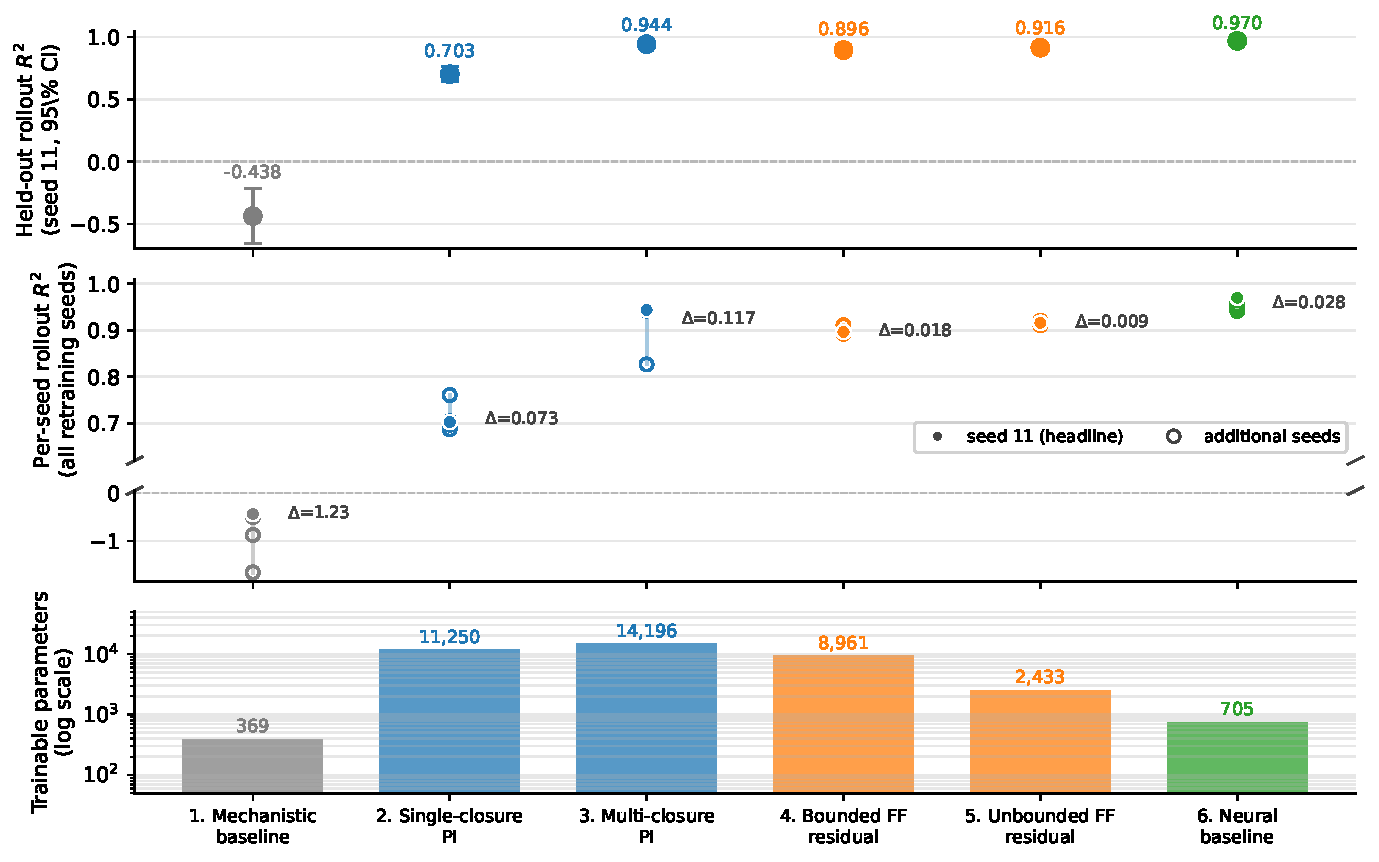
\includegraphics[width=\linewidth]{figures/position_spectrum.pdf}
\caption{Placement spectrum across the six model classes (Table~\ref{tab:rollout_summary}). \textbf{Top:} Held-out autonomous-rollout $R^2$ at seed 11 with 95\% roast-bootstrap CI. The mechanistic baseline anchors the spectrum near $R^2 = -0.44$; every PIML repair strategy lifts the rollout above $0.70$, and the matched-input neural baseline reaches the highest accuracy at $R^2 = 0.97$. \textbf{Middle:} \rev{Per-seed rollout $R^2$ across all evaluated retraining seeds (five per class, six where available; \Methods) with the range $\Delta$ annotated; filled markers are the seed-11 headline runs. The vertical axis is split so that seed-level variation among the repaired classes remains resolvable alongside the mechanistic baseline's much larger spread. The multi-closure PI is the highest-R$^2$ physics-informed repair but also the least seed-stable ($\Delta = 0.117$, one of six seeds finishing far below the others); both FF-residual variants are the tightest ($\Delta \le 0.018$).} \textbf{Bottom:} Trainable-parameter count (log scale). Every PIML repair uses at least three times the parameters of the neural baseline. Colors mark the placement of the MLP relative to the ODE: gray for none, blue for inside the ODE, orange for on top of the ODE rollout, green for standalone.}
\label{fig:position_spectrum}
\end{figure}

\begin{figure}[!htbp]
\centering
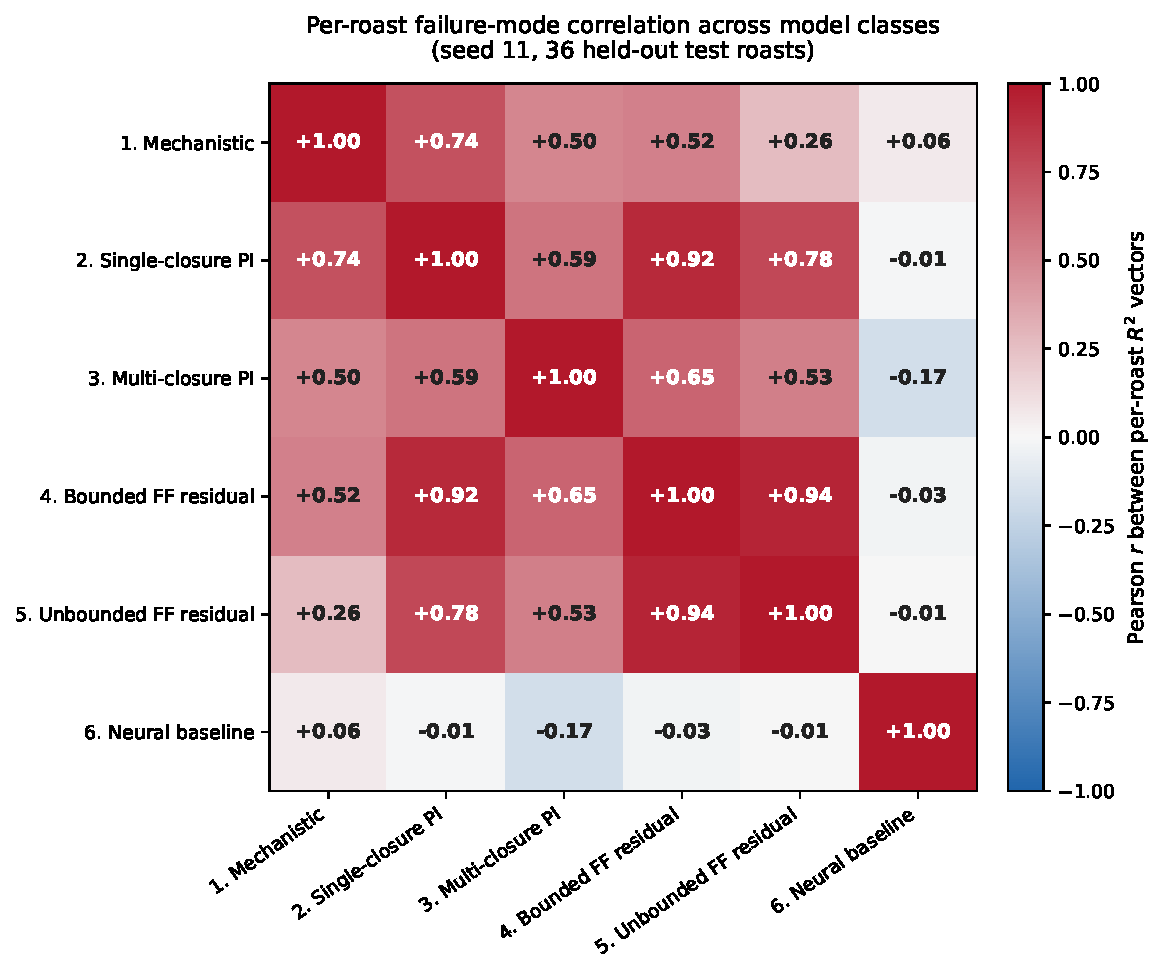
\includegraphics[width=0.85\linewidth]{figures/per_roast_correlation_heatmap.pdf}
\caption{Pearson correlation between per-roast rollout $R^2$ vectors across the six model classes (seed 11, 36 held-out test roasts). The four PIML repair strategies (rows/columns 2--5) form a high-correlation block ($r \approx 0.5$--$0.9$), indicating that they share their hard roasts with one another. The matched-input neural baseline (row/column 6) is the dark-band exception: its per-roast hardness is near-orthogonal to every PIML repair ($|r| \le 0.17$), so the two approaches reach a comparable predictive ceiling through structurally different per-roast failure profiles.}
\label{fig:per_roast_corr}
\end{figure}

\begin{figure}[!htbp]
\centering
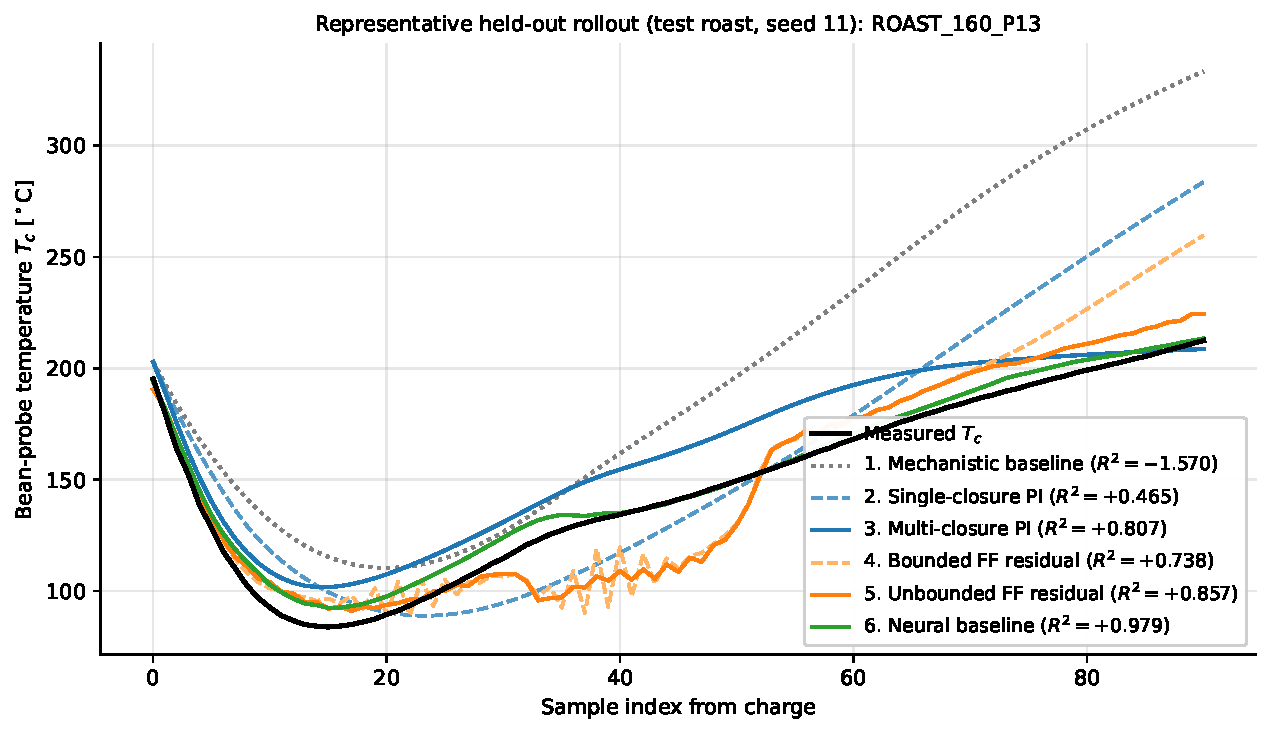
\includegraphics[width=\linewidth]{figures/representative_rollouts.pdf}
\caption{Representative held-out rollout on the deterministic-longest test roast (seed 11) for all six model classes in the placement spectrum (Table~\ref{tab:rollout_summary}). The measured bean-probe trace is shown in black. Mechanistic baseline (gray dotted) drifts substantially upward after the charge-drop transient. Within each repair location, the two variants are paired by linestyle: single-closure PI (dashed blue) and multi-closure PI (solid blue) for inside-the-ODE repair; bounded FF residual (dashed orange) and unbounded FF residual (solid orange) for on-top-of-ODE repair. The matched-input neural baseline (green) tracks the measured trajectory most closely. Per-roast rollout $R^2$ values for this specific roast are annotated in the legend and may differ from the cohort-pooled values in Table~\ref{tab:rollout_summary}.}
\label{fig:representative_rollouts}
\end{figure}

\begin{figure}[!htbp]
\centering
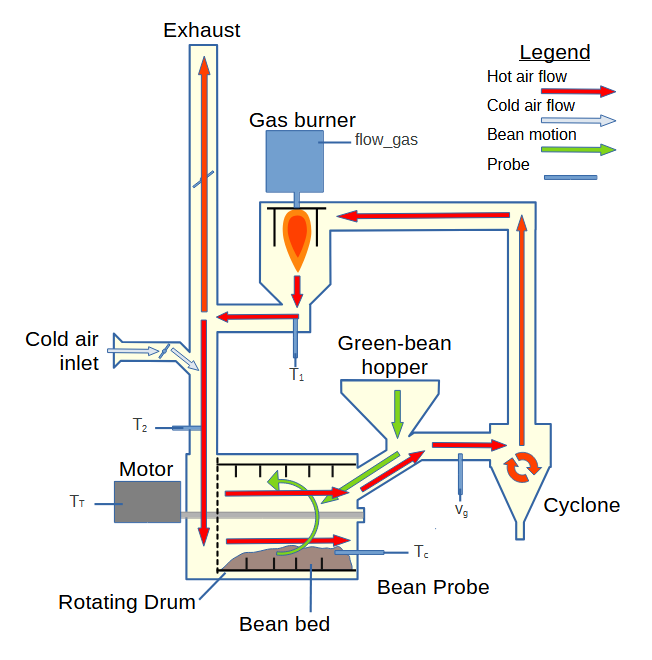
\includegraphics[width=\linewidth]{figures/roaster_schematic_3.png}
\caption{\rev{Schematic of the industrial roaster configuration and the placement of the measured signals used in this study (original drawing by the authors). Green coffee is charged from the hopper into the preheated rotating drum, where the bean bed is heated by hot process air and drum contact; the process-air loop runs from the gas burner through the drum and cyclone, with partial recirculation into the burner duct and the remainder vented through the exhaust. Labeled markers show the six telemetry signals of the canonical data schema (\Methods, Table~\ref{tab:symbols}): the bean-probe temperature $T_c$, measured by a probe positioned near the bulk bean bed and used as the modeled output, and the drum-inlet air temperature $T_2$, air-speed signal $v_g$, and drum rotation speed $T_T$ drive the models at every step, while the burner-outlet temperature $T_1$ and burner gas-flow command \texttt{flow\_gas} enter only the initial-state inference at charge. The production telemetry contains additional plant tags beyond those shown; only the labeled signals enter the reported models. Bean discharge and downstream cooling equipment are omitted because the modeled window ends when the beans leave the drum.}}
\label{fig:roast_process}
\end{figure}

\begin{figure}[!htbp]
\centering
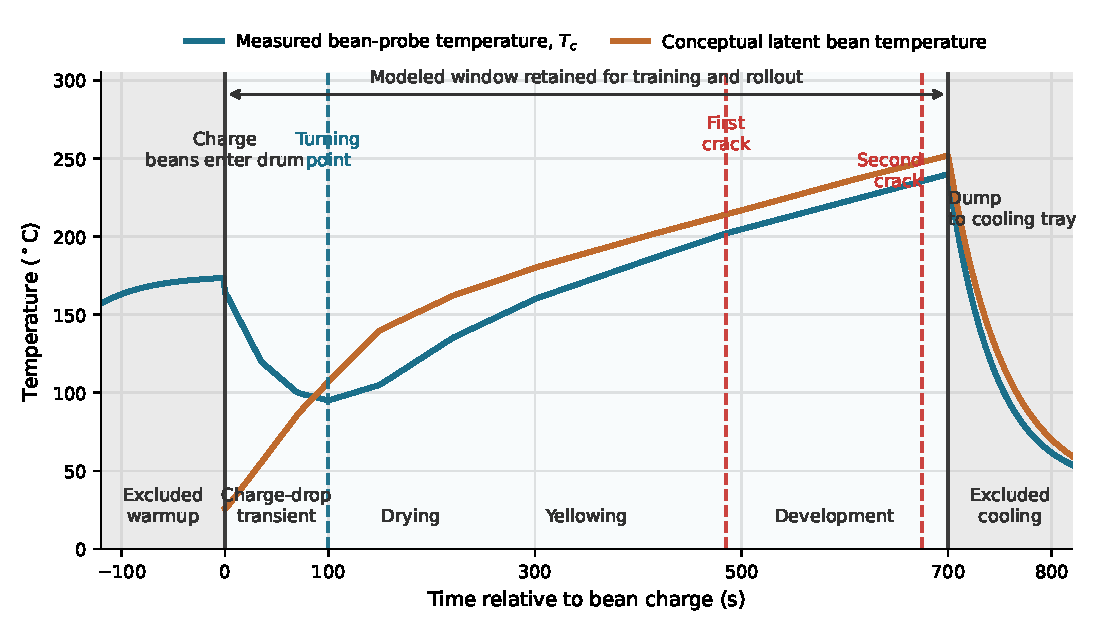
\includegraphics[width=\linewidth]{figures/roast_profile_preprocessing_schematic.pdf}
\caption{Schematic roasting profile and preprocessing window used in the experiments. The measured bean-probe temperature $T_c$ is the modeled output. The latent bean-temperature curve is included only as process context and is not directly measured in the production telemetry. Pre-charge warmup and post-dump cooling are excluded from the model sequences, while the charge-drop transient, turning point, and later roast development are retained in the charge-to-dump modeled window. Crack markers indicate common roast-stage landmarks rather than inputs used by the reported models.}
\label{fig:roast_profile_preprocessing}
\end{figure}

\begin{table}[!htbp]
\centering
\small
\begin{tabular}{|l|c|c|c|c|c|}
\hline
Placement / model & Where the MLP plugs in & Rollout $R^2$ & 95\% CI & RMSE [$^\circ$C] & Params \\
\hline
1.~Mechanistic baseline & none (mechanistic only) & $-0.4376$ & $[-0.6551,\,-0.2164]$ & 41.79 & 369 \\
2.~Single-closure PI & inside ODE ($h_e$ only) & $0.7027$ & $[0.6480,\,0.7611]$ & 19.00 & 11{,}250 \\
3.~Multi-closure PI & inside ODE (three relations) & $0.9436$ & $[0.9165,\,0.9717]$ & 8.28 & 14{,}196 \\
4.~Bounded FF residual & on top of ODE, $\pm 24$~K bound & $0.8963$ & $[0.8566,\,0.9386]$ & 11.23 & 8{,}961 \\
5.~Unbounded FF residual & on top of ODE, no bound & $0.9158$ & $[0.8869,\,0.9468]$ & 10.11 & 2{,}433 \\
6.~Neural baseline & standalone (no ODE) & $0.9697$ & $[0.9560,\,0.9805]$ & 6.07 & 705 \\
\hline
\end{tabular}
\caption{Held-out autonomous-rollout metrics on the 221-roast production cohort, seed 11. Each model class was tuned by an independent 40-trial validation-rollout random search and then retrained at the manuscript-canonical training budget across \rev{five or six retraining seeds (\Methods)}; reported values are seed 11. Intervals are 95\% roast-bootstrap intervals for pooled rollout $R^2$. The six placements vary by \emph{where} a feedforward MLP is plugged in relative to the mechanistic ODE: none (row 1), inside the ODE as one or three learned closure terms (rows 2--3), on top of the ODE rollout as a bounded or unbounded additive correction (rows 4--5), or standalone with no physics (row 6).}
\label{tab:rollout_summary}
\end{table}

\begin{table}[!htbp]
\centering
\small
\begin{tabular}{|p{0.36\linewidth}|p{0.38\linewidth}|c|}
\hline
Model component & Architecture & Neural parameters \\
\hline
Shared initial-state network (all PI variants) & $6 \rightarrow 32 \rightarrow 4$ & 356 \\
PI single-closure MLP ($h_e$) & $3 \rightarrow 128 \rightarrow 64 \rightarrow 32 \rightarrow 1$ & 10{,}881 \\
Multi-closure PI: $h_e$ MLP & $3 \rightarrow 128 \rightarrow 64 \rightarrow 32 \rightarrow 1$ & 10{,}881 \\
Multi-closure PI: moisture-rate MLP & $2 \rightarrow 32 \rightarrow 16 \rightarrow 1$ & 641 \\
Multi-closure PI: reaction-rate MLP & $2 \rightarrow 64 \rightarrow 32 \rightarrow 1$ & 2{,}273 \\
Bounded FF residual MLP & $4 \rightarrow 128 \rightarrow 64 \rightarrow 1$ & 8{,}961 \\
Unbounded FF residual MLP & $4 \rightarrow 64 \rightarrow 32 \rightarrow 1$ & 2{,}433 \\
Matched-input neural baseline MLP & $4 \rightarrow 32 \rightarrow 16 \rightarrow 1$ & 705 \\
\hline
\end{tabular}
\caption{Neural parameter counts for the learned components after hyperparameter selection. Architectures are the winning configurations from each model class's 40-trial validation-rollout random search. Every learned component is a feedforward MLP; the comparison axis in Table~\ref{tab:rollout_summary} is therefore where the MLP plugs in relative to the mechanistic ODE, not what kind of network is used. The mechanistic and physics-informed scaffolds additionally include $\sim$13 learned scalar physical parameters (initial-state offsets, effective contact area, kinetic prefactors and activation energies, probe time-constant, heat of vaporization, total reaction heat); those scalars are not included in the counts above.}
\label{tab:model_capacity}
\end{table}

\begin{table}[!htbp]
\centering
\small
{\color{blue}
\begin{tabular}{|l|p{0.42\linewidth}|l|l|}
\hline
Symbol & Physical meaning & Units & Status \\
\hline
\multicolumn{4}{|l|}{\emph{Measured telemetry}} \\
\hline
$T_c$ & Bean-probe temperature (modeled output) & $^{\circ}$C & measured \\
$T_2$ ($\equiv T_{gi}$ in the equations) & Inlet roasting-air temperature entering the drum & $^{\circ}$C & measured driver \\
$v_g$ & Air-speed signal forming the gas-side flow term & m\,s$^{-1}$ & measured driver \\
$T_T$ & Drum rotation speed & rpm & measured driver \\
$T_1$ & Burner-outlet air temperature (initial-state inference only) & $^{\circ}$C & measured \\
\texttt{flow\_gas} & Burner gas-flow command (initial-state inference only) & \% & measured \\
$\Delta t$ & Per-roast telemetry sample interval & s & measured \\
\hline
\multicolumn{4}{|l|}{\emph{Latent model states (equation~\eqref{eq:state}) and algebraic intermediates}} \\
\hline
$T_b$ & Latent bulk bean temperature & $^{\circ}$C & latent state \\
$X_b$ & Bean moisture ratio (dry basis) & kg\,kg$^{-1}$ & latent state \\
$H_e$ & Accumulated exothermic reaction energy & J\,kg$^{-1}$ & latent state \\
$T_{rp}$ & Modeled probe temperature (compared to $T_c$) & $^{\circ}$C & latent state \\
$T_{go}$ & Latent outlet-air temperature & $^{\circ}$C & algebraic \\
$T_g$ & Internal gas-temperature proxy supplied by the mechanistic rollout; input to the learned closures & $^{\circ}$C & algebraic \\
$G_g$ & Gas-side mass flow, $A_{\mathrm{air}}\rho_g v_g$ & kg\,s$^{-1}$ & algebraic \\
$\phi_{gb},\,\phi_r,\,\phi_{ev}$ & Gas-to-bean, reaction, and evaporative heat flows & W & algebraic \\
\hline
\multicolumn{4}{|l|}{\emph{Learned scalar physical parameters (13 total)}$^{\dagger}$} \\
\hline
$h_e$ & Effective gas-to-bean heat-transfer coefficient & W\,m$^{-2}$\,K$^{-1}$ & learned$^{\ddagger}$ \\
$A_b$ & Effective bean contact area & m$^2$ & learned \\
$m_{b,\mathrm{dry}}$ & Effective dry bean mass & kg & learned \\
$A_{\mathrm{air}}$ & Effective air-duct flow area & m$^2$ & learned \\
$k_X$ & Moisture-loss rate prefactor & s$^{-1}$ & learned \\
$E_X$ & Moisture-loss activation temperature ($E/R$ form) & K & learned \\
$A_r$ & Exothermic reaction-rate prefactor & J\,kg$^{-1}$\,s$^{-1}$ & learned \\
$E_r$ & Reaction activation temperature ($E/R$ form) & K & learned \\
$H_{e,\mathrm{tot}}$ & Total exothermic energy capacity & J\,kg$^{-1}$ & learned \\
$h_v$ & Latent heat of moisture vaporization & J\,kg$^{-1}$ & learned \\
$k_p$ & Probe first-order response time constant & s$^{-1}$ & learned \\
--- & Global initial bean-temperature offset from first probe sample & $^{\circ}$C & learned \\
--- & Global initial-moisture parameter (logit) & --- & learned \\
\hline
\multicolumn{4}{|l|}{\emph{Fixed literature properties}} \\
\hline
$\rho_g$ & Air density & kg\,m$^{-3}$ & fixed \\
$c_{pg}$ & Air specific heat (polynomial in gas temperature) & J\,kg$^{-1}$\,K$^{-1}$ & fixed function \\
$c_{pb}$ & Bean specific heat (function of $X_b$) & J\,kg$^{-1}$\,K$^{-1}$ & fixed function \\
\hline
\end{tabular}
\caption{Symbols of the mechanistic scaffold (equations~\eqref{eq:state}--\eqref{eq:probe}) and the learned-closure input $T_g$ (equation~\eqref{eq:single_closure}): physical meaning, units, and status. $^{\dagger}$Learned scalars are parameterized as log-scale multipliers on literature base values and initialized at the literature value (scale~1); the two initial-state scalars are the exception described in \Methods, parameterizing a telemetry-referenced initial-state guess. $^{\ddagger}$In the physics-informed variants, $h_e$ is replaced by the learned closure of equation~\eqref{eq:single_closure}; in the multi-closure variant the moisture-loss and reaction rates are additionally replaced by the learned closures of equation~\eqref{eq:multi_closure}.}
\label{tab:symbols}
}
\end{table}

\end{document}
